\chapter{Implementation Approach}\label{chap:Methodology}

This project reuses and extends the Terraform module structure already built in earlier
weeks (the subnet module, the OKE module) rather than rebuilding infrastructure from
scratch. In this chapter, we explain the mechanisms that make that configuration
reusable across five services and safe to extend, and the pipeline that carries a code
change from a service repository into the running cluster.

\section{Building on the Existing Terraform Foundation}\label{sec:manual-console-build}
Rather than a manual, console-first build, this project's starting point was the
already-validated \texttt{network} and \texttt{oke} Terraform modules from earlier
weeks. The root module (\texttt{Terraform-code/main.tf}) wires them together, resolves
the latest Oracle Linux image for the chosen compute shape, and provisions one OCIR
repository per microservice from a single \texttt{for\_each}:

\begin{lstlisting}[caption={\texttt{Terraform-code/main.tf} -- one resource block, five OCIR repositories}]
resource "oci_artifacts_container_repository" "microservices" {
  for_each = local.microservices

  compartment_id = var.compartment_ocid
  display_name   = "shared-group-a-cmp/${each.value}"
  is_public      = false
  is_immutable   = false
}
\end{lstlisting}

\texttt{local.microservices} is the set \texttt{auth-service}, \texttt{products-service},
\texttt{orders-service}, \texttt{payments-service}, and \texttt{ecomm-ui}. Adding a sixth
service later means adding one entry to that set, not writing a new resource block.

\subsection*{Module Interfaces}
The \texttt{network} and \texttt{oke} modules are wired together strictly through typed
inputs and outputs, not through any shared state outside Terraform. Figures~\ref{fig:network-module}
and~\ref{fig:oke-module} set out each module's contract.

\begin{figure}[H]
\centering
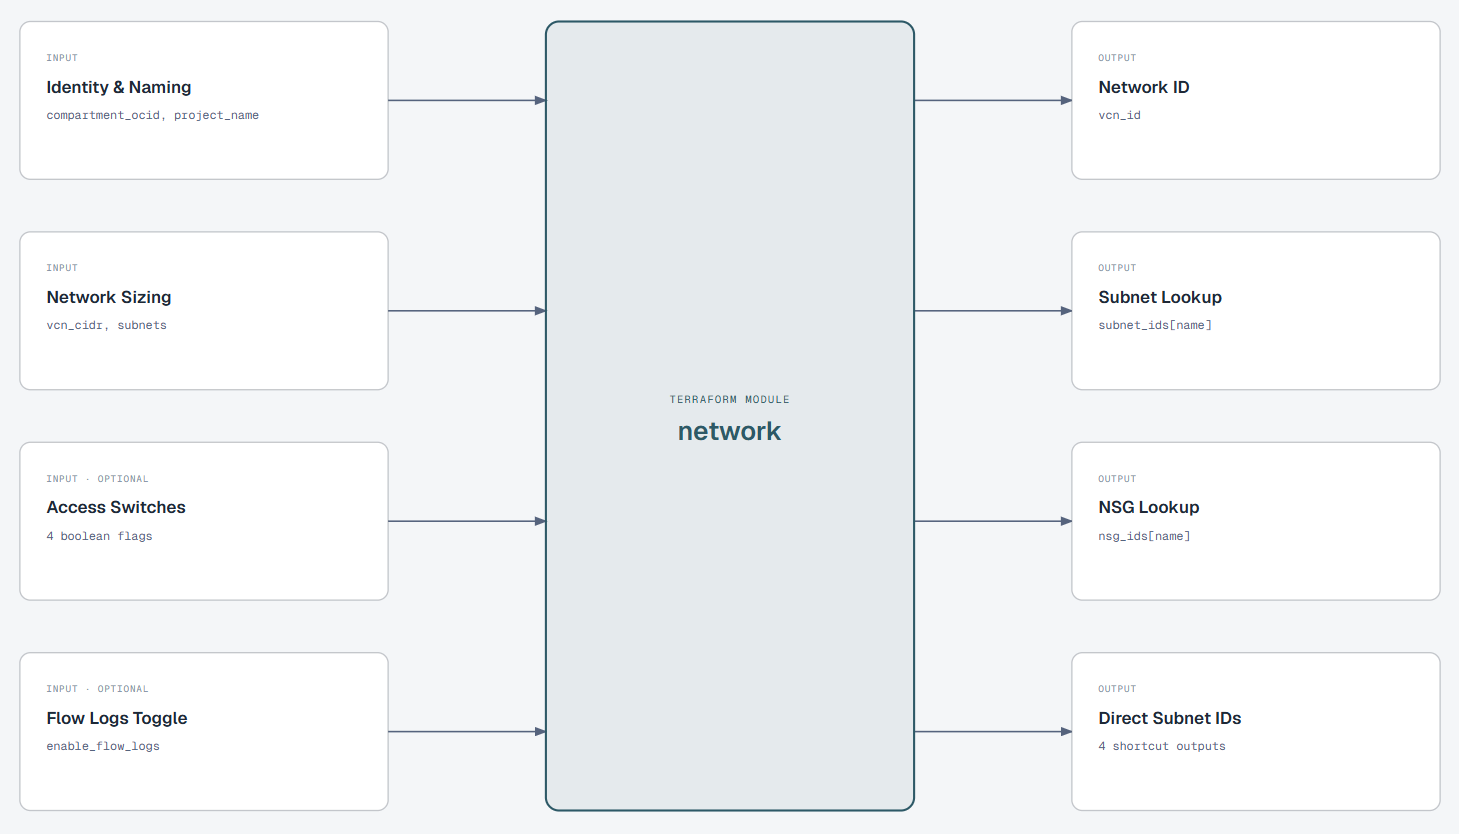
\includegraphics[width=0.92\textwidth]{Figures/networkModuleInterface.png}
\caption{Interface of the \texttt{network} module. Required inputs fix identity/naming
and network sizing; four boolean access switches and a flow-log toggle are optional.
Outputs expose the VCN ID plus by-name lookup maps for subnets and NSGs, alongside four
shortcut outputs for the individual subnet IDs.}
\label{fig:network-module}
\end{figure}

\begin{figure}[H]
\centering
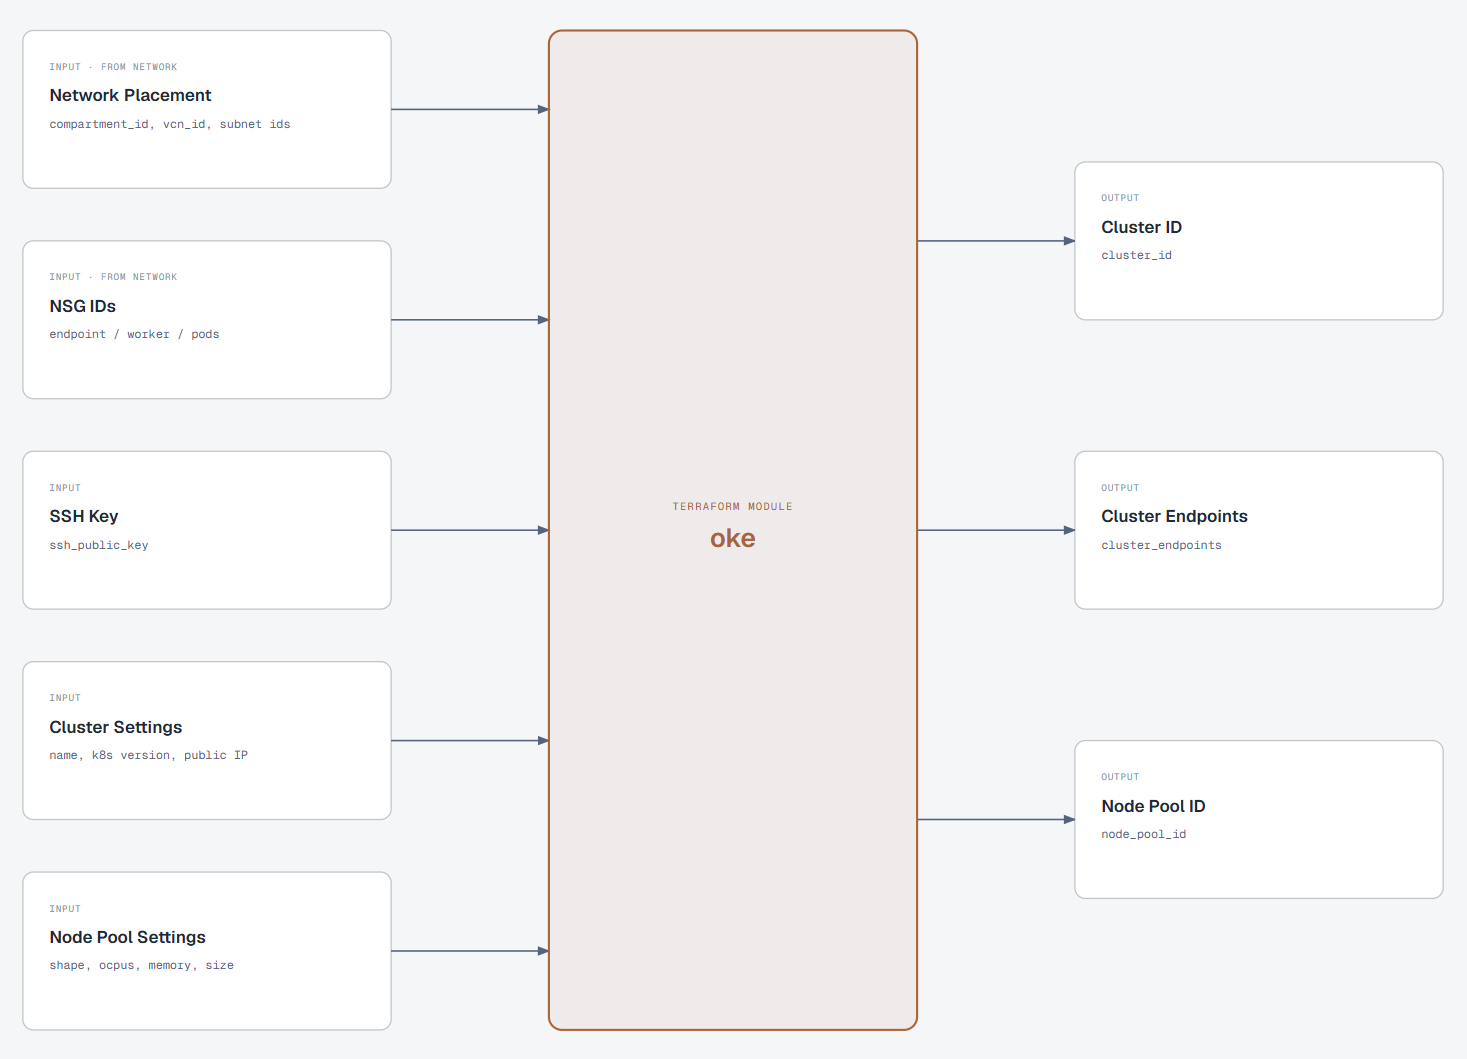
\includegraphics[width=0.92\textwidth]{Figures/okeModuleInterface.png}
\caption{Interface of the \texttt{oke} module. Two of its inputs, network placement and
NSG IDs, are consumed directly from the \texttt{network} module's outputs rather than
declared independently, which is what makes the root module's
\texttt{module.oke \{ vcn\_id = module.network.vcn\_id, ... \}} wiring possible. The
remaining inputs (SSH key, cluster settings, node pool settings) are root-level
variables. Outputs expose the cluster ID, its API endpoints, and the node pool ID.}
\label{fig:oke-module}
\end{figure}

This input/output discipline is what lets the root module wire \texttt{oke} to
\texttt{network} with a handful of direct output-to-input references
(\texttt{vcn\_id}, the subnet IDs, the NSG IDs), without either module reaching into
the other's internal resources.

\section{Implementation Method: Configuration and Inputs}\label{sec:research-method}
Table~\ref{tab:variables} lists the inputs the root Terraform module accepts.

\begin{table}[H]
\centering
\caption{Selected variables declared in \texttt{Terraform-code/variable.tf}.}
\label{tab:variables}
\small
\begin{tabularx}{\textwidth}{>{\raggedright\arraybackslash}p{3.4cm} l
                >{\raggedright\arraybackslash}X}
\toprule
\textbf{Variable} & \textbf{Type} & \textbf{Purpose} \\
\midrule
\code{compartment\_\allowbreak ocid} & string & Target compartment (required, no default) \\
\code{region} & string & OCI region (required, no default) \\
\code{node\_shape} & string & OKE worker node compute shape, default \code{VM.Standard.A1.Flex} \\
\code{node\_ocpus} & number & OCPUs per worker node, default \code{2} \\
\code{node\_\allowbreak memory\_\allowbreak in\_\allowbreak gbs} & number & Memory per worker node, default \code{16} \\
\code{node\_count} & number & Worker nodes per availability domain, default \code{2}, floored at \code{2} regardless of input \\
\code{ssh\_public\_key} & string & SSH public key for optional worker node troubleshooting access \\
\code{github\_token}, \code{github\_owner}, \code{github\_repo} & string, sensitive & Credentials used to write the OKE cluster OCID back into GitHub Actions secrets \\
\bottomrule
\end{tabularx}
\end{table}

\section{Configuration Framework: Reducing Repetition}\label{sec:analytical-framework}
The network module's NSG rules are the clearest example of avoiding repetition in this
configuration. Every ingress and egress rule, for every subnet, is declared once as data
in \texttt{modules/network/locals.tf}, then flattened into a single map keyed by
\texttt{"<subnet>-<index>"} so one \code{for\_each} can generate every rule resource:

\begin{lstlisting}[caption={\texttt{modules/network/locals.tf} -- flattening per-subnet rule lists into one for\_each-able map}]
ingress_rules_flat = merge([
  for nsg_key, rules in local.ingress_by_nsg : {
    for idx, rule in rules :
    "${nsg_key}-${idx}" => merge(rule, { nsg_key = nsg_key })
  }
]...)
\end{lstlisting}

Adding a seventh ingress rule to any subnet means adding one object to the relevant list
in \texttt{ingress\_by\_nsg}; the resource block that actually creates
\texttt{oci\_core\_network\_security\_group\_security\_rule} resources never changes.
The same \texttt{for\_each} pattern is used for the four subnets themselves, each built
from a typed \texttt{map(object(\{cidr\_block, is\_public\}))} variable rather than four
separate resource blocks.

\section{Change-Safety: Promoting One Service at a Time}\label{sec:evaluation-criteria}
Because each microservice has its own repository, its own CI pipeline, and its own entry
in the Helm chart's \texttt{values.yaml}, changing one service's image does not require
touching Terraform or the other four services. Table~\ref{tab:change-criteria} sets out
how a change actually reaches the cluster.

\begin{table}[H]
\centering
\caption{How a code change in one service reaches the running cluster.}
\label{tab:change-criteria}
\small
\begin{tabularx}{\textwidth}{>{\raggedright\arraybackslash}p{3.6cm}
                >{\raggedright\arraybackslash}X}
\toprule
\textbf{Step} & \textbf{What happens} \\
\midrule
Push to \texttt{main} in a service repository & That repository's own \texttt{ci.yml} builds the Docker image and pushes it to OCIR, tagged with both the GitHub Actions run number and \texttt{latest} \\
Reusable \texttt{update-helm.yml} workflow & Checks out \texttt{Terraform-code}, converts the service's dash-case name to the matching \texttt{values.yaml} key, and uses \texttt{yq} to bump only that service's \texttt{image.tag} \\
Commit and push to \texttt{Terraform-code} & The updated \texttt{values.yaml} is committed back to the Helm chart's repository \\
ArgoCD reconciliation & ArgoCD's automated sync (prune and self-heal enabled) detects the change and rolls out the new image for that one deployment \\
\bottomrule
\end{tabularx}
\end{table}

Because \texttt{update-helm.yml} only ever edits one service's \texttt{image.tag} key,
promoting \texttt{payments-service} cannot accidentally change what image
\texttt{auth-service} is running. Figure~\ref{fig:pipeline-flow} shows the same sequence
as a single left-to-right path.

\begin{figure}[H]
\centering
\resizebox{\textwidth}{!}{%
\begin{tikzpicture}[node distance=14mm]
\node[outputbox, text width=26mm] (push) {\textbf{Push}\\{\scriptsize to \texttt{main}}};
\node[evalbox, right=of push, text width=32mm] (ci) {\textbf{ci.yml}\\{\scriptsize build + push image}};
\node[neutralbox, right=of ci, text width=24mm] (ocir) {\textbf{OCIR}\\{\scriptsize tagged image}};
\node[evalbox, right=of ocir, text width=34mm] (helm) {\textbf{update-\allowbreak helm.yml}\\{\scriptsize bump \texttt{values.yaml}}};
\node[outputbox, right=of helm, text width=30mm] (argocd) {\textbf{ArgoCD}\\{\scriptsize sync + self-heal}};
\draw[arrow] (push) -- (ci);
\draw[arrow] (ci) -- (ocir);
\draw[arrow] (ocir) -- (helm);
\draw[arrow] (helm) -- (argocd);
\end{tikzpicture}
}
\caption{The image-promotion pipeline as one path: a push to a single service's
repository ends, four steps later, in ArgoCD rolling out only that service's new
image.}
\label{fig:pipeline-flow}
\end{figure}

\section{Container Image Build and Health Checks}\label{sec:container-build}
Every backend service is built from the same two-stage Dockerfile pattern, shown here
for \texttt{auth-service}:

\begin{lstlisting}[language={}, caption={\texttt{auth-service/Dockerfile}}]
FROM node:20-alpine AS builder
WORKDIR /app
COPY package*.json ./
RUN npm ci || npm install
COPY . .

FROM node:20-alpine AS runner
WORKDIR /app
ENV NODE_ENV=production
COPY --chown=node:node --from=builder /app /app
USER node
EXPOSE 5001

HEALTHCHECK --interval=30s --timeout=5s --start-period=10s --retries=3 \
  CMD wget --no-verbose --tries=1 --spider http://localhost:5001/health || exit 1

CMD ["npm", "start"]
\end{lstlisting}

The builder stage installs dependencies and copies source; the runner stage copies only
the finished \texttt{/app} directory forward and switches to the non-root \texttt{node}
user before starting the process, so the container never runs as root. Each service
exposes its own \texttt{/health} endpoint (a plain 200 response, no dependency checks),
which both the Docker-level \texttt{HEALTHCHECK} and the Kubernetes liveness and
readiness probes target.

The four backend services (\texttt{auth-service}, \texttt{products-service},
\texttt{orders-service}, \texttt{payments-service}) use the same probe timing in their
Kubernetes manifests, set out in Table~\ref{tab:health-probes}.

\begin{table}[H]
\centering
\caption{Liveness and readiness probe timing, common to the four backend services.}
\label{tab:health-probes}
\small
\begin{tabularx}{\textwidth}{>{\raggedright\arraybackslash}p{3cm} X X}
\toprule
\textbf{Probe} & \textbf{Initial delay / period / timeout} & \textbf{Failure threshold} \\
\midrule
Liveness (\texttt{GET /health}) & 15s initial delay, every 10s, 5s timeout & 3 consecutive failures restart the container \\
Readiness (\texttt{GET /health}) & 5s initial delay, every 5s, 3s timeout & 3 consecutive failures remove the pod from Service routing \\
\bottomrule
\end{tabularx}
\end{table}

The readiness probe's shorter delay and interval mean a pod is pulled out of rotation
quickly if it stops responding, while the liveness probe's longer thresholds avoid
restarting a container that is merely slow to start.

\section{Records as the Source of Truth}\label{sec:data-evidence-weighting}
Two records anchor this system, at two different layers. Terraform's own state file is
the source of truth for the infrastructure it manages: the VCN, subnets, NSGs, the OKE
cluster, and the OCIR repositories. Above that, once the cluster exists, the Helm chart's
\texttt{values.yaml} inside \texttt{Terraform-code} is the source of truth for
\emph{which image tag each workload is currently running}, and ArgoCD's own sync status
is the record of whether the live cluster actually matches that file. This is the core
GitOps property the pipeline in Section~\ref{sec:evaluation-criteria} relies on: the
desired state lives in Git, not on any one operator's machine.

\section{Assumptions and Limitations}\label{sec:assumptions-limitations}
Two decisions were left open in the assessment phase and resolved with concrete defaults
during the Terraform build rather than being specified upfront: the OKE node pool's
compute shape and OCPU/memory split defaulted to \texttt{VM.Standard.A1.Flex} at 2 OCPUs
and 16\,GB of memory, and the specific database engine per service was resolved by
running a single shared MongoDB instance for all five services rather than one database
per service. We revisit both as open items in Chapter~\ref{chap:concl}. Separately, the
root module's IAM policy resources (a dynamic group and policy that would let OKE worker
nodes pull images and read secrets without a static auth token) are present in
\texttt{main.tf} but commented out, with an inline note that the team did not have
tenancy-level access to create dynamic groups in this environment; an OCIR auth token
is used instead.

\section{Environment Teardown}\label{sec:environment-teardown}
The deployment runbook (\texttt{Terraform-code/DEPLOYMENT.md}) documents teardown in
dependency order, uninstalling the application before destroying the infrastructure that
hosts it:

\begin{lstlisting}[style=shellstyle, caption={Teardown sequence from DEPLOYMENT.md}]
helm uninstall ecommerce -n ecommerce-ns
kubectl delete -f ./Project/Terraform-code/kubernetes/

cd /home/ali_hamad/terraform/Project/Terraform-code
terraform destroy
\end{lstlisting}

The application layer (Helm release or raw manifests) is removed first, then the
underlying OKE cluster and network are destroyed through Terraform.
